\documentclass[11pt]{article}
\usepackage[margin=1in]{geometry}
\usepackage{amsmath,amssymb,booktabs,graphicx,xcolor}
\usepackage[colorlinks=true,linkcolor=blue,citecolor=blue,urlcolor=blue]{hyperref}
\title{\textbf{peaches}: ChEES-adapted ensemble HMC\\[2pt]
\large A reproducible benchmark of the Hamiltonian walk move vs.\ \texttt{emcee}
and NUTS}
\author{}
\date{}

\begin{document}
\maketitle

\begin{abstract}
\noindent
\textsc{peaches} is the \emph{Hamiltonian walk move} --- an affine-invariant
ensemble HMC proposal whose metric is the empirical covariance of the live
ensemble --- with its integration length tuned by the \textbf{ChEES} criterion
(Change in the Estimator of the Expected Square; Hoffman, Radul \& Sountsov,
AISTATS 2021) and its step size by Nesterov dual averaging (Hoffman \& Gelman,
JMLR 2014). We benchmark it against \texttt{emcee} (the gradient-free
affine-invariant stretch move; Goodman \& Weare 2010, Foreman-Mackey et al.\
2013) and NUTS (\texttt{numpyro}) on controlled targets with exact moments, over
three axes: dimensional scaling, conditioning vs.\ curvature, and warmup
robustness. Every run is checked for convergence (rank-normalized split
$\hat R$), and every reported efficiency is a median over the \emph{converged}
seeds only; all configurations and commands are given for exact reproduction.
\end{abstract}

% =====================================================================
\section*{Overview}

\textsc{peaches} combines three ingredients, and the three benchmarks below each
isolate one. \textbf{(i)} Its preconditioner is the \emph{empirical covariance of
the live ensemble}, recomputed every step, so --- exactly like \texttt{emcee} ---
it is affine-invariant: linear ill-conditioning is handled \emph{for free}, with
no mass matrix to fit (Exp.~2a) and no mass-matrix warmup to pay for (Exp.~3).
\textbf{(ii)} It integrates \emph{gradient} Hamiltonian dynamics, so --- unlike
\texttt{emcee} --- it crosses position-dependent curvature (Exp.~2b) and follows
the optimal-HMC dimensional-scaling law (Exp.~1). \textbf{(iii)} Its trajectory
length is tuned online by ChEES and its step size by dual averaging, so it is
turn-key. The four axes below --- dimension, conditioning, curvature, warmup ---
are exactly the four places single-strategy samplers fail, and \textsc{peaches}
is the only one here that clears all four at once:

\begin{center}\small
\renewcommand{\arraystretch}{1.2}
\begin{tabular}{@{}lllll@{}}
\toprule
Axis (experiment) & what it stresses & \textsc{peaches} & \texttt{emcee} & NUTS \\
\midrule
Dimension (Exp.~1) & cost growth with $d$
  & $d^{-1/4}$ (optimal) & $d^{-1}$ & $d^{-1/4}$ \\
Conditioning (Exp.~2a) & linear anisotropy $\kappa$
  & flat (free) & flat (free) & flat \emph{only} w/ mass adapt. \\
Curvature (Exp.~2b) & nonlinear ridge
  & crosses it & fails ($\hat R\!\to\!2$) & crosses it \\
Warmup (Exp.~3) & tuning cost
  & flat from $w{=}50$ & --- & needs $w\gtrsim500$ \\
\bottomrule
\end{tabular}
\end{center}

\noindent
\texttt{emcee} is affine-invariant but gradient-free, so it dies on both
dimension and curvature; NUTS integrates gradients but must \emph{fit} a mass
matrix, so it needs a long warmup and, without it, loses conditioning-robustness.
\textsc{peaches} inherits the ensemble metric from the first and gradient dynamics
from the second, and pays for neither.

% =====================================================================
\section{Methods}\label{sec:methods}

\paragraph{\textsc{peaches}: a ChEES-adapted Hamiltonian walk move.}
Let the ensemble be $W$ walkers $q_{1:W}\in\mathbb{R}^d$ with target
$\pi(q)\propto e^{-U(q)}$. The \emph{Hamiltonian walk move} (``h-walk'')
proposes a Hamiltonian trajectory for a subset of walkers using a momentum that
lives in the span of the \emph{complement} ensemble: with $C$ the centered
complement walkers (rows $q_j-\bar q$), momentum $p$ is a $W\!\times\!W$ matrix
and the leapfrog updates are
\[
q \leftarrow q + \epsilon\, p\,C,\qquad
p \leftarrow p - \epsilon\, \nabla U(q)\,C^{\!\top},
\]
so positions move only within the affine subspace spanned by the ensemble and
the effective metric is the empirical ensemble covariance
$\Sigma=\mathrm{cov}(C)$. This makes the move \emph{affine-invariant}: it is
unchanged under any invertible linear reparametrization of $q$, so its
efficiency is independent of the target's conditioning. (A complementary
``h-side'' move proposes along a single random ensemble difference direction;
both are Metropolis-corrected with the standard HMC accept ratio.) The
preconditioner is recomputed from the live ensemble \emph{every iteration} ---
there is no separately-fit mass matrix.

\paragraph{Adaptation (warmup only).} Three independently-toggleable adapters
run during warmup and are then frozen:
\begin{enumerate}
\item \emph{Initial step size} via a heuristic line search
(\texttt{find\_init\_step\_size}): double/halve $\epsilon$ until the first
trajectory's acceptance brackets the target.
\item \emph{Step size} $\epsilon$ via Nesterov dual averaging (Hoffman \& Gelman
2014) toward a target acceptance (we pin $0.8$ for the scaling law). The
log-step update uses gain $\sqrt{t}/\gamma$ on the running acceptance error
$\bar H$; the realized acceptance is the harmonic mean of per-walker
$\min(1,e^{\log\alpha})$.
\item \emph{Integration length} $T=\epsilon L$ via the \textbf{ChEES} criterion
(Hoffman et al.\ 2021). ChEES does ADAM ascent on the expected change in
squared jump distance: the per-step gradient signal is
$g \propto h_t\,T\,(\lVert c_{\text{pro}}\rVert_\Sigma^2 -
\lVert c_{\text{cur}}\rVert_\Sigma^2)\,(c_{\text{pro}}^{\!\top}\Sigma^{-1} v)$,
where $c$ are centered positions, $v$ the trajectory velocity, $h_t$ a Halton
sequence, and $\lVert\cdot\rVert_\Sigma$ the \emph{affine-invariant}
$\Sigma^{-1}$ norm (matching the move's metric). ADAM ($\beta_1{=}0$,
$\beta_2{=}0.95$, lr $0.025$, per-step clip $\pm0.35$) updates $\log T$; the
realized length is Halton-jittered, $L=\lceil T/\epsilon\rceil$ capped at
$L_{\max}$.
\end{enumerate}
Setting all three flags off reduces warmup to a plain burn-in at a fixed
$(\epsilon,L)$. \textsc{peaches} thus realizes \emph{optimally-tuned} ensemble
HMC: the metric is free (the ensemble), the step size hits a target acceptance,
and the trajectory length maximizes squared jump distance.

\paragraph{Baselines.} \texttt{emcee} is the gradient-free affine-invariant
stretch move (Goodman \& Weare 2010; \texttt{emcee}, Foreman-Mackey et al.\
2013): it is exactly affine-invariant like the h-walk but uses \emph{no}
gradient. NUTS is \texttt{numpyro}'s implementation with window mass-matrix
adaptation; we use the mass matrix appropriate to each experiment (\S below) and
also an \emph{ablation} with the mass fixed to the identity
(\texttt{adapt\_mass\_matrix=False}) to isolate the role of preconditioning.

\paragraph{Targets, metric, convergence.} Targets are the isotropic Gaussian
$N(0,I_d)$, the rotated ill-conditioned Gaussian (condition number
$\kappa=e^{\log\kappa}$), and the Rosenbrock banana --- all with exact moments.
Efficiency is \emph{production-only} ESS per \textbf{target evaluation} (worst
coordinate): this counts one \emph{gradient} per leapfrog step for the gradient
samplers (\textsc{peaches}, NUTS) and one \emph{log-density} per walker per
iteration for gradient-free \texttt{emcee} --- the fair per-oracle-call cost in
each case. Throughout we use the \emph{ensemble-mean} ESS estimator: the
integrated autocorrelation of the walker-averaged series, rescaled by the pooled
variance ratio. This is the natural estimator for an interacting ensemble and is
$O(dN\log N)$ --- no per-walker FFT --- so it stays cheap even at the thousands
of walkers the scaling sweep reaches (it agrees with ArviZ's rank-normalized ESS
to within the mild antithetic boost of well-tuned HMC, $\lesssim\!25\%$).
Ensemble methods use $n_{\text{walkers}}=8d$ --- a \emph{constant} $8$ walkers
per dimension (floor $64$), so the empirical covariance and the ChEES
trajectory-length estimate are equally well-resolved at every $d$
(\S\ref{sec:scaling}) --- except the fixed-$d$ warmup experiment, where any
full-rank count suffices ($400$ at $d{=}100$). Ensemble runs also use a stretch
pre-warmup (\S\ref{sec:rec}).
\textbf{Convergence is enforced throughout}: each per-dimension point is the
median over its \emph{converged} seeds (rank-normalized split $\hat R\le1.03$;
relaxed slightly from $1.01$ for seed-median plus thinning noise, all genuine
failures sit at $\hat R\ge1.04$), a stuck seed never enters the median, and a
point is drawn solid only if a \emph{majority} of its seeds converged (hollow
otherwise --- a hollow point's ESS/eval is not a meaningful efficiency).

% =====================================================================
\section{Experiment 1 --- dimensional scaling}\label{sec:scaling}

\begin{figure}[h]
\centering
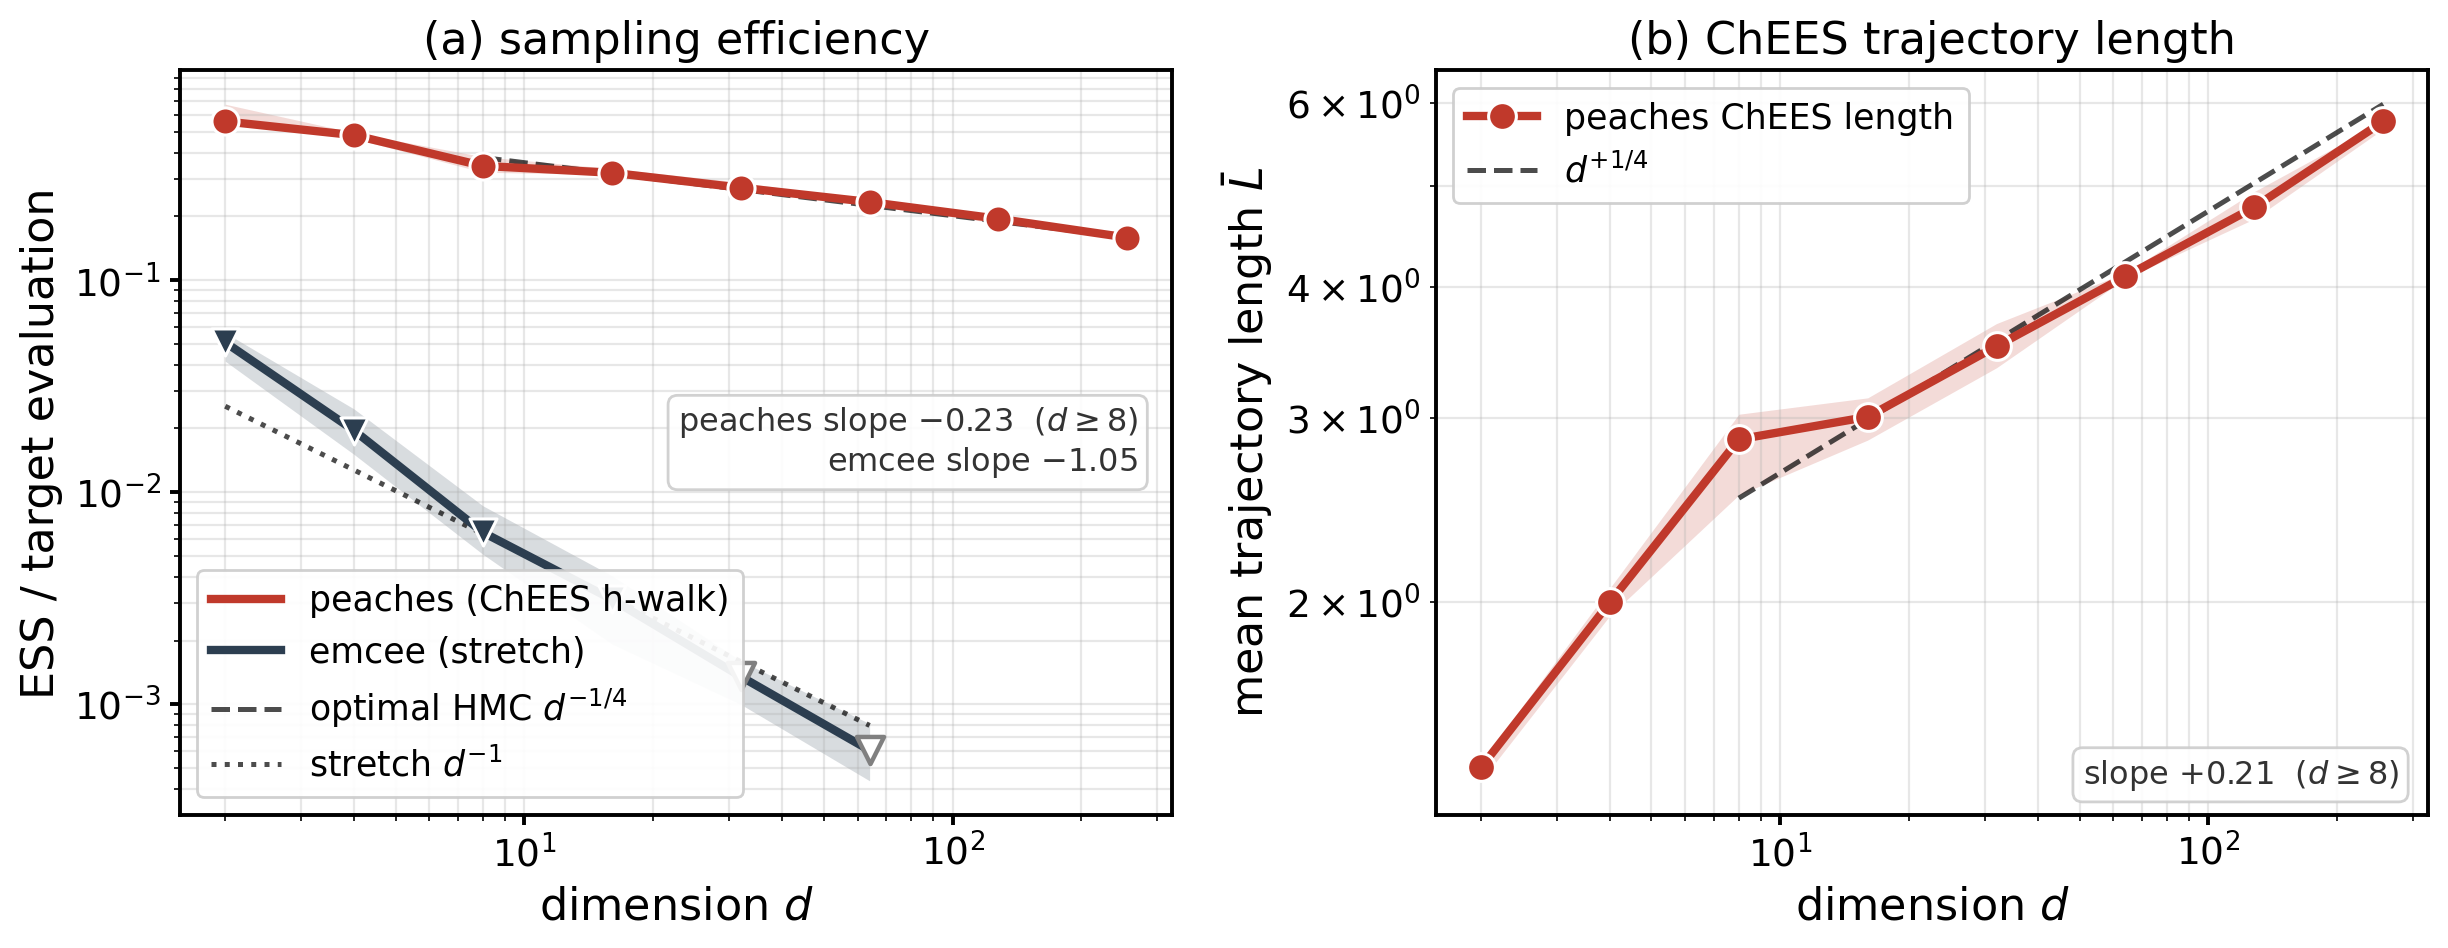
\includegraphics[width=\linewidth]{figs/pn_scaling.png}
\caption{Isotropic Gaussian $N(0,I_d)$, $d=2$--$256$, constant
$n_{\text{walkers}}=8d$ (floor $64$), $5$ seeds ($3$ at $d{=}256$), ensemble-mean
ESS. Median over the converged seeds; band = seed min--max. \textbf{(a)} sampling
efficiency: \textsc{peaches} is a clean monotone optimal-HMC $d^{-1/4}$ law
across the whole range (fitted slope $-0.23$ for $d\ge8$, theory $-0.25$), while
\texttt{emcee} falls as $d^{-1}$ (fitted $-1.05$) --- an exponentially widening
gap ($\sim\!11\times$ at $d{=}2$, $\sim\!380\times$ at $d{=}64$). \textbf{(b)} the
mechanism: \textsc{peaches}'s ChEES-tuned mean trajectory length grows smoothly
as $d^{+1/4}$ (fitted $+0.21$), the signature of the $\epsilon\sim d^{-1/4}$
step-size law. Holding the walkers-per-dimension ratio fixed at $8$ is what makes
both panels smooth: the ChEES length estimate is then equally well-resolved at
every $d$, with no low-$d$ over-integration. (NUTS also achieves $d^{-1/4}$ and is
omitted here so the peaches-vs-emcee contrast reads cleanly; it is benchmarked in
\S\ref{sec:cond}--\ref{sec:warmup}.)}
\label{fig:scaling}
\end{figure}

\paragraph{Setup.} Target $N(0,I_d)$ (\texttt{--no-rotate --log-cond 0}) for
$d\in\{2,4,\dots,256\}$, constant $n_{\text{walkers}}=8d$ (floor $64$), $5$ seeds
($3$ at $d{=}256$; tag \texttt{scale3}). \textsc{peaches} pins
\texttt{--target-accept 0.8} so the step-size law holds at a fixed acceptance;
stretch pre-warmup $w_s{=}100$, warmup $4000$ (long enough for dual averaging to
converge), production $5000$ ($3000$ at $d\ge128$; ESS/eval is a ratio,
insensitive to production length once converged), $L_{\max}=512$. Runs are scored
with the fast ensemble-mean ESS (\texttt{--fast-ess}), which makes even the
$2048$-walker $d{=}256$ cell cheap. \texttt{emcee} mixes far more slowly, so it is
run much longer --- warmup $3000$, production $1.2\!\times\!10^4$ --- and shown
only where it reaches $\hat R\le1.03$ ($d\le64$). On the paired Rosenbrock
($d{=}2$--$32$, Fig.~\ref{fig:rosen}) \textsc{peaches} uses the same constant
$8d$ walker rule (floor $64$), warmup $8000$, $8$ seeds (tag \texttt{rz8}), and
\texttt{emcee} the same walkers (tag \texttt{rz8}).

\paragraph{Result.} Optimally-tuned HMC needs $\epsilon\sim d^{-1/4}$ at fixed
acceptance, hence $L\sim d^{1/4}$ and $\text{ESS}/\text{eval}\sim d^{-1/4}$
(Beskos et al.\ 2013). \textsc{peaches} realizes this cleanly across the whole
range: the fitted efficiency slope is $-0.23$ ($d\ge8$; theory $-0.25$) and
$\bar L$ grows as $d^{+1/4}$ (fitted $+0.21$, $\bar L$ from $1.4$ at $d{=}2$ to
$5.8$ at $d{=}256$). The key is holding the walkers-per-dimension ratio
\emph{constant} at $8$: the optimal length is small in low dimensions
($d^{1/4}\!<\!2$), and resolving it requires that the empirical covariance ---
and hence the ESJD gradient ChEES ascends --- be well-estimated. At a fixed $8d$
walkers it is well-estimated at \emph{every} $d$, so ChEES adapts the correct
short $\bar L$ throughout and the efficiency is a smooth monotone decline with no
low-$d$ hump. (At a fixed $4d$ the covariance is too noisy in low $d$; ChEES then
over-integrates --- $\bar L\!\approx\!6$ where $\le\!3$ is optimal --- and the
per-eval efficiency is spuriously suppressed, producing a low-$d$ artefact.)
\texttt{emcee}'s gradient-free stretch move scales as
$\text{ESS}/\text{eval}\sim d^{-1}$ (fitted $-1.05$ over the converged
$d\in[8,64]$); already at $d{=}64$ \textsc{peaches} is $\sim\!380\times$ more
efficient per target evaluation, the gap widens exponentially in $d$, and
\texttt{emcee} cannot be converged at all beyond $d{=}64$ in a feasible run.

\begin{figure}[h]
\centering
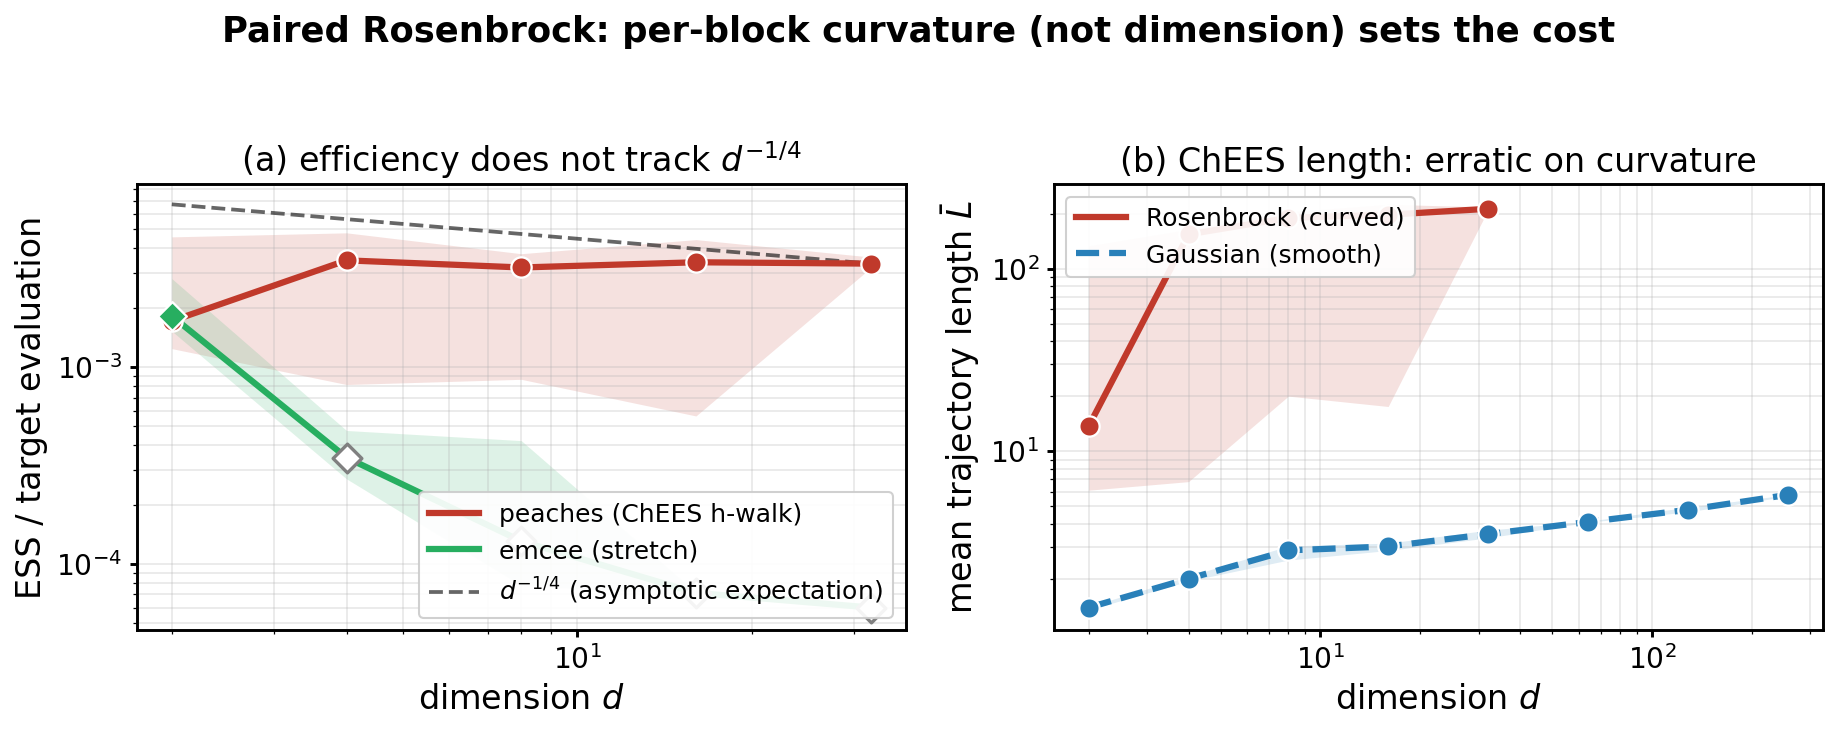
\includegraphics[width=\linewidth]{figs/pn_rosen.png}
\caption{Dimensional scaling on the \emph{paired} Rosenbrock (a product of $d/2$
identical banana pairs). Median over the converged seeds, band = seed min--max;
hollow = a minority of seeds converged. \textbf{(a)} \textsc{peaches} stays
efficient ($\text{ESS}/\text{eval}\sim10^{-3}$) and converges, but does \emph{not}
fall as $d^{-1/4}$ (dashed reference) --- it drifts upward; \texttt{emcee} fails to
converge for $d\ge4$. \textbf{(b)} the mechanism: \textsc{peaches}'s ChEES length
is large and erratic on the curved banana ($\bar L\!\sim\!10$--$220$, bimodal
across seeds) but smooth on the Gaussian ($\bar L\!\sim\!2$--$9$, short in low
$d$, growing as $d^{1/4}$); the curvature, not the dimension, sets the cost.}
\label{fig:rosen}
\end{figure}

\paragraph{Rosenbrock --- the law is masked by curvature.} The paired Rosenbrock
is formally a product of $d/2$ identical banana pairs, so in principle it obeys
the same $d^{-1/4}$ law. It does not over the accessible range $d\le32$
(Fig.~\ref{fig:rosen}a). \textsc{peaches} converges (where \texttt{emcee} cannot)
and stays efficient ($\text{ESS}/\text{eval}\!\sim\!10^{-3}$), but the curve is
seed-variable and does not fall as $d^{-1/4}$. The cause (Fig.~\ref{fig:rosen}b)
is the per-block curvature: it gives ChEES no single good integration length, so
the adapted $\bar L$ is \emph{bimodal} --- a long trajectory that traverses a
banana ($\bar L\!\sim\!200$) or a short stuck one ($\bar L\!\sim\!15$) --- versus
the Gaussian's smooth $\bar L$. This bimodality is not a mere nuisance: it is a
genuine, reproducible \textbf{failure mode of trajectory-length adaptation on
curved targets}, it sets the whole cost, and --- as we show next --- it is
invisible to the usual $\hat R$ convergence check. We therefore dissect it in
\S\ref{sec:bistab}; the robust curvature statement is the qualitative $2\times2$
of \S\ref{sec:cond}, not a power law.

% =====================================================================
\section{A ChEES failure mode: trajectory-length bistability on curvature}
\label{sec:bistab}

\begin{figure}[h]
\centering
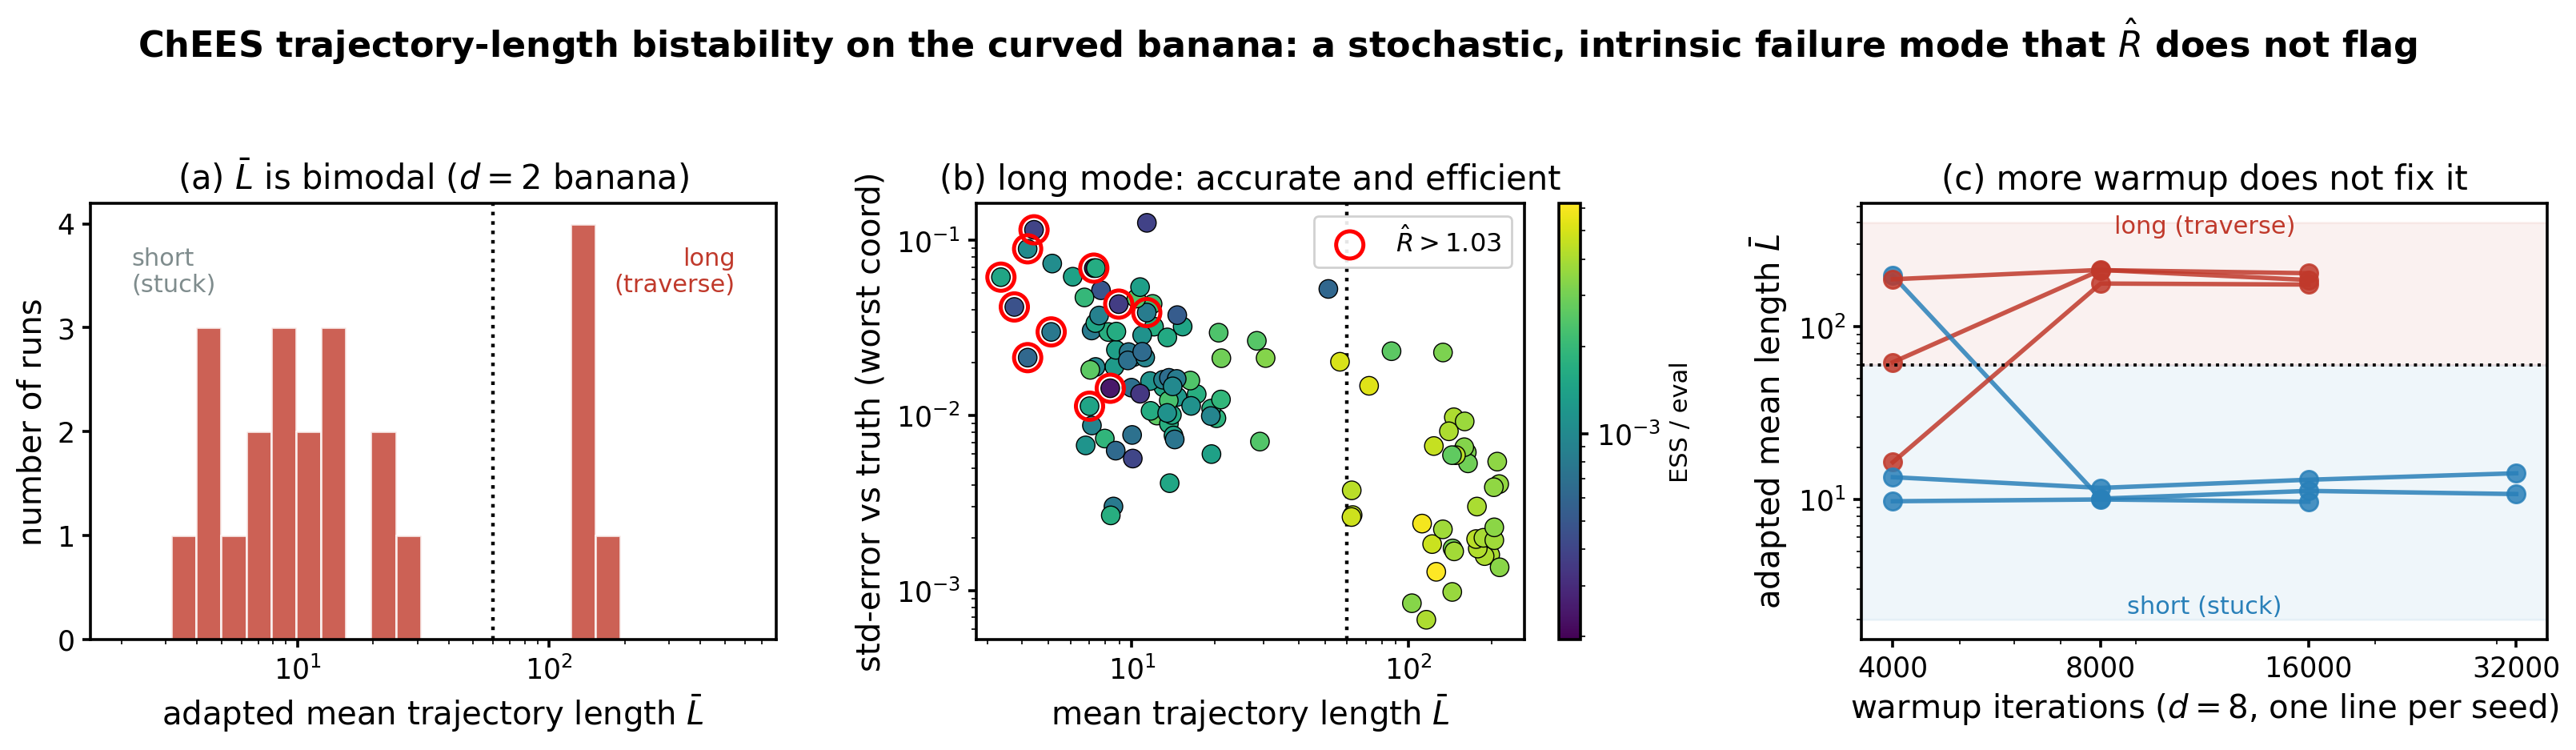
\includegraphics[width=\linewidth]{figs/pn_bistability.png}
\caption{ChEES trajectory-length \emph{bistability} on the banana, characterised
on the cheap $d{=}2$ single banana (which already carries the curvature) and
corroborated at $d{=}8$. \textbf{(a)} across many seeds the adapted $\bar L$ is
sharply \emph{bimodal} --- a short ``stuck'' mode ($\bar L\!\lesssim\!30$) and a
long ``ridge-traversing'' mode ($\bar L\!\gtrsim\!100$), with a clean gap.
\textbf{(b)} the long mode is better on \emph{both} axes at once --- lower error
vs.\ the exact moments \emph{and} higher ESS/eval (colour) --- so this is a
good-vs-stuck split, not a speed/accuracy trade-off; crucially, almost every run
passes rank-split $\hat R\le1.03$ (only the few red-ringed points fail), so
\textbf{$\hat R$ does not separate the modes}. \textbf{(c)} tracking each $d{=}8$
seed's adapted $\bar L$ as warmup grows $4000\!\to\!32000$: seeds sit in the long
(red) or short (blue) mode and \emph{stay} there --- one even drifts
long$\to$short with \emph{more} warmup --- so the split is intrinsic and
stochastic, not an under-tuning artefact that a longer warmup removes.}
\label{fig:bistab}
\end{figure}

\paragraph{Setup.} $d{=}2$ Rosenbrock (one banana), $64$ walkers,
\texttt{--max-L 512}, \texttt{--target-accept 0.8}, production $8000$, scored with
the ensemble ESS; up to $24$ seeds per cell (tags \texttt{b2\_w$w$\_i$s$}). We
also varied the initialisation scale over $\{0.5,1,2,4\}$, which did not
systematically shift the long/short fraction. The $d{=}8$ corroboration
(Fig.~\ref{fig:bistab}c) fixes $256$ walkers and sweeps warmup
$\{4000,8000,16000,32000\}$ across $6$ seeds (tag \texttt{rwarm\_w$w$}).

\paragraph{Result --- an intrinsic, $\hat R$-invisible bistability.}
On the curved ridge the ChEES objective (expected squared jump distance under the
ensemble metric) has \emph{two} self-consistent fixed points, and the
adapted length collapses onto one or the other (Fig.~\ref{fig:bistab}a, a clean
bimodal histogram). The two are \emph{not} equivalent: the long mode traverses a
banana in one trajectory and is simultaneously the more \emph{accurate} (median
std-error vs.\ truth $\approx0.003$ vs.\ $\approx0.02$ for the short mode) and
the more \emph{efficient} ($\text{ESS}/\text{eval}\approx4\times10^{-3}$ vs.\ $1\times10^{-3}$);
the short mode is genuinely \emph{stuck}, under-exploring a banana arm
(Fig.~\ref{fig:bistab}b). The alarming part is that the stuck mode still passes
the standard convergence check: its median rank-split $\hat R$ is only
$\approx1.01$ and $\sim\!87\%$ of stuck runs sit below the usual $1.03$
threshold, so a practitioner watching $\hat R$ alone would accept a run with
several-fold larger error and $\sim\!4\times$ lower efficiency as converged.

\paragraph{Why is each mode \emph{stable}? A state-dependent objective.} The
surprise is not that ChEES can pick a poor length once, but that the poor length
is a \emph{stable} attractor that longer tuning does not escape. The reason is
that the ChEES objective is not fixed: it maximises ESJD in the \emph{ensemble
covariance} $\Sigma^{-1}$ norm, and $\Sigma$ is recomputed from the live walkers
every step, so the length and the metric co-evolve. This closes a self-reinforcing
loop with two fixed points. \emph{Long}: a large $L$ makes trajectories traverse
and spread \emph{along} the banana ridge, so $\Sigma$ elongates along it, and
ESJD in that elongated norm is maximised by long traversals --- which keeps $L$
large ($\mathrm{IAT}\!\approx\!1$: one trajectory decorrelates). \emph{Short}: a
small $L$ keeps the walkers local, so $\Sigma$ stays compact and
\emph{under-dispersed} (hence the $\sim\!8\times$ larger std-error), and in that
compact norm even a short step already looks like a large normalised jump ---
which keeps $L$ small ($\mathrm{IAT}\!\approx\!90$). Tellingly, the two modes
share essentially the \emph{same} dual-averaged step size ($\epsilon\!\approx\!
0.03$) and acceptance ($\approx\!0.93$): the step-size adapter and the acceptance
criterion cannot tell them apart, only the length differs. Because ChEES ascends a
\emph{local} gradient (ADAM on $\log T$), it cannot tunnel between basins, and the
co-adapting metric locks in whichever basin the early warmup fell into --- classic
multistability of an adaptive scheme whose objective depends on the state it has
itself produced.

\paragraph{The sharp gap is a fingerprint of the $\Sigma^{-1}$ norm.} If the
state-dependent metric is what sharpens the split, replacing it should blur the
gap. It does. Re-running the $d{=}2$ study with ChEES measuring ESJD in a
\emph{fixed Euclidean} norm (\texttt{--chees-metric euclidean}, i.e.\ the
identity matrix in place of $\Sigma^{-1}$; the h-walk move itself is unchanged)
turns the cleanly bimodal $\bar L$ (short $3$--$30$, long $123$--$160$, empty in
between) into a broad \emph{continuum} ($\bar L\!=\!4,5,\dots,22,38,49,62,66,
\dots,161$): the intermediate lengths that the $\Sigma^{-1}$ feedback forbade are
now populated. This is the predicted signature --- the sharp two-attractor
structure comes from the metric co-adapting with the length. But the Euclidean
variant is not a fix: its efficiency and error are no better (it still produces
short, stuck runs, because Euclidean ESJD is a poor proxy for mixing on the
curved ridge), and it \emph{forfeits the affine-invariance} that the $\Sigma^{-1}$
norm exists to provide (\S\ref{sec:cond}a). The bistability is thus an intrinsic
tension of trajectory-length adaptation on curvature, not an artefact of one norm
choice.

\paragraph{It is not under-tuning.} A natural hypothesis is that the short mode is
simply a warmup that has not finished adapting. It is not
(Fig.~\ref{fig:bistab}c): quadrupling the warmup ($8000\!\to\!32000$) leaves the
long-mode fraction essentially unchanged, individual $d{=}8$ seeds stay stuck
short at every warmup length tested (and some even flip long$\to$short with
\emph{more} warmup), and varying the initialisation scale over $8\times$ does not
move the fraction either. The basin a run lands in is a stochastic property of
the coupled ensemble--ChEES dynamics on the curved geometry, not a transient. The
practical remedy is therefore not ``warm up longer'' but \textbf{(i)} monitor an
error/accuracy diagnostic (or the adapted $\bar L$ itself) alongside $\hat R$,
which \emph{does} separate the modes, and \textbf{(ii)} prefer a leaner ensemble,
which we found lands in the long mode more often. That the whole phenomenon
reproduces on the two-dimensional banana --- where it costs seconds to study ---
makes it a clean, cheap test case for trajectory-length adapters on curvature.

% =====================================================================
\section{Experiment 2 --- conditioning vs.\ curvature}\label{sec:cond}

\begin{figure}[h]
\centering
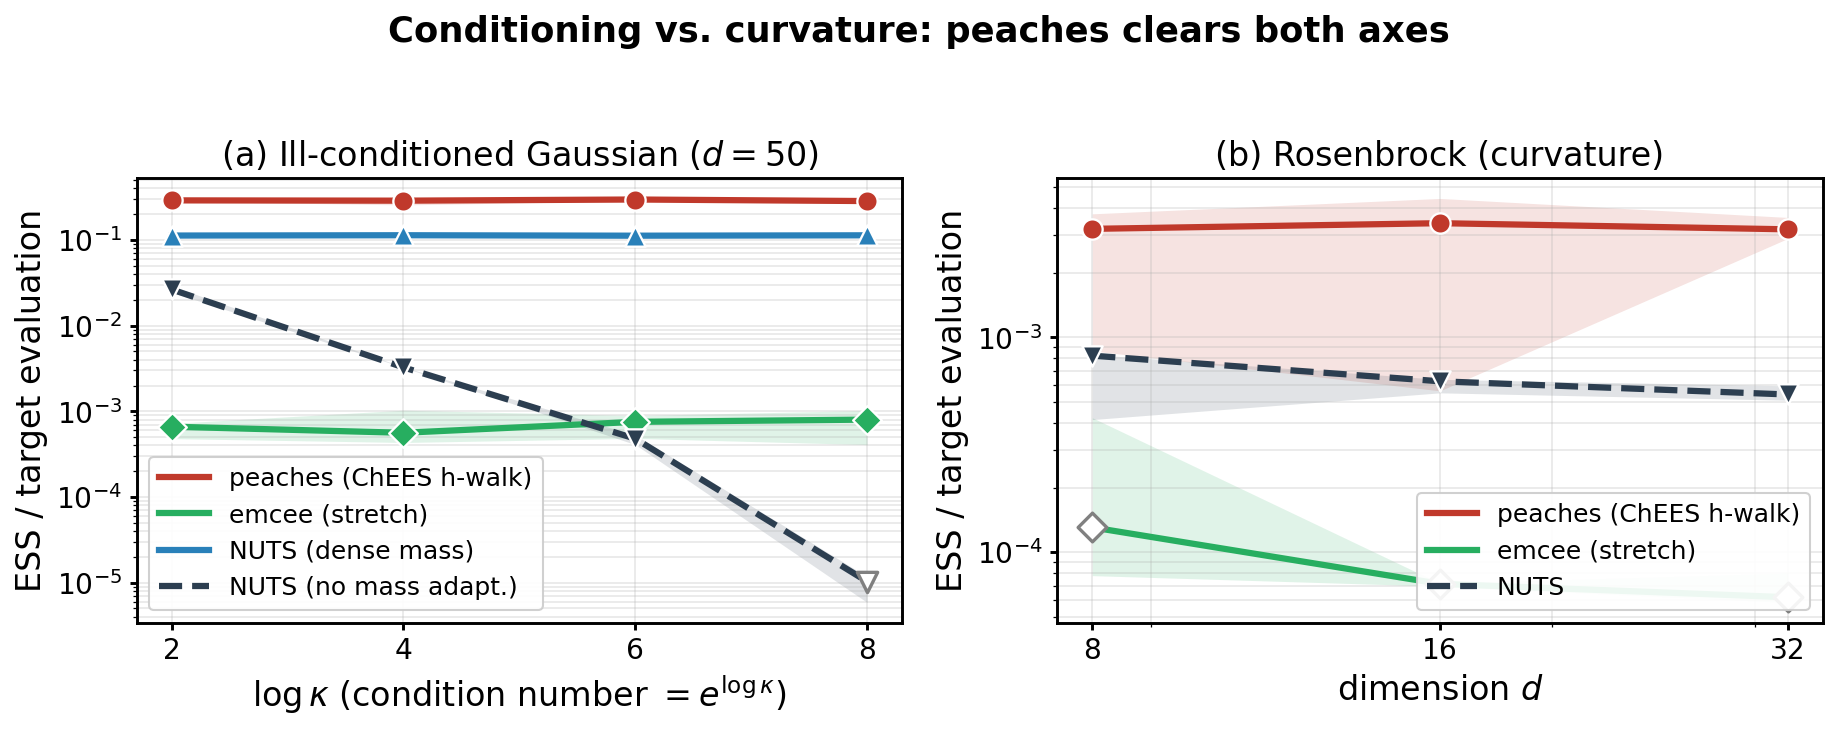
\includegraphics[width=\linewidth]{figs/pn_conditioning.png}
\caption{Two targets isolate two failure modes; only \textsc{peaches} clears
both. Median over converged seeds, band = seed min--max; solid = converged
($\hat R\le1.03$), hollow = not. \textbf{(a) conditioning} --- Gaussian $d{=}50$
vs.\ $\kappa$: \textsc{peaches} and \texttt{emcee} are flat because their metric
is the ensemble covariance; NUTS is flat \emph{only} through mass adaptation ---
fix its mass to the identity and efficiency collapses $4$ orders. \textbf{(b)
curvature} --- Rosenbrock vs.\ $d$: the gradient methods (\textsc{peaches}, NUTS)
integrate along the curved ridge and stay converged; \texttt{emcee}'s single
affine map cannot, and it fails to converge for $d\ge4$. Takeaway: the ensemble
metric buys conditioning-robustness for free, gradient dynamics buy
curvature-handling, and \textsc{peaches} has both.}
\label{fig:cond}
\end{figure}

\paragraph{Setup.} (a) Rotated Gaussian $d{=}50$, $\kappa=e^{2,4,6,8}$, warmup
$1000$, $8d{=}400$ walkers (the scaling rule); \textsc{peaches} (production
$5000$, tag \texttt{condf\_lc$k$}), \texttt{emcee} (production $4\!\times\!10^4$),
NUTS dense-mass (\texttt{condf\_lc$k$}, the standard sampler) and NUTS
identity-mass (\texttt{--nuts-mass identity}, production $2000$, tag
\texttt{condfid\_lc$k$}, the ablation). (b) Rosenbrock $d\in\{8,16,32\}$, $8d$
walkers (tag \texttt{rz8}): \textsc{peaches} ($L_{\max}=512$), \texttt{emcee},
NUTS identity-mass (tag \texttt{rz8id}). On Rosenbrock the global conditioning is
mild, so mass adaptation is irrelevant and the identity-mass NUTS represents NUTS
faithfully. All runs are scored with the ensemble ESS.

\paragraph{Result --- a clean $2\times2$.} The two targets isolate two distinct
failure modes. \emph{Conditioning} (panel a): the empirical-covariance metric
makes \textsc{peaches} and \texttt{emcee} affine-invariant, so their ESS/eval is
flat in $\kappa$ ($\approx\!0.29$ and $\approx\!7\times10^{-4}$, the latter just
dimensionally penalised at $d{=}50$). NUTS is flat in $\kappa$ \emph{only}
through its mass adaptation: with the mass fixed to the identity its ESS/eval
falls from $2.6\times10^{-2}$ ($\kappa=e^2$) to $5.9\times10^{-6}$
($\kappa=e^8$) --- over four orders, and unconverged ($\hat R\!\approx\!1.06$) at
$\kappa=e^8$.
\emph{Curvature} (panel b): Rosenbrock's position-dependent curvature defeats
any fixed linear map. \texttt{emcee}'s single affine stretch move cannot cross
the ridge --- even at $10^5$ samples it fails to converge for $d\ge4$
($\hat R$ grows $1.14\!\to\!2.0$ over $d{=}8\!\to\!32$). \textsc{peaches} and
NUTS integrate \emph{local} Hamiltonian dynamics along the ridge and stay
converged ($\text{ESS}/\text{eval}\approx10^{-3}$). Only \textsc{peaches} clears
both axes: the ensemble preconditioner gives it the conditioning-robustness
un-adapted NUTS lacks, and gradient dynamics give it the curvature-handling
\texttt{emcee} lacks.

% =====================================================================
\section{Experiment 3 --- warmup robustness}\label{sec:warmup}

\begin{figure}[h]
\centering
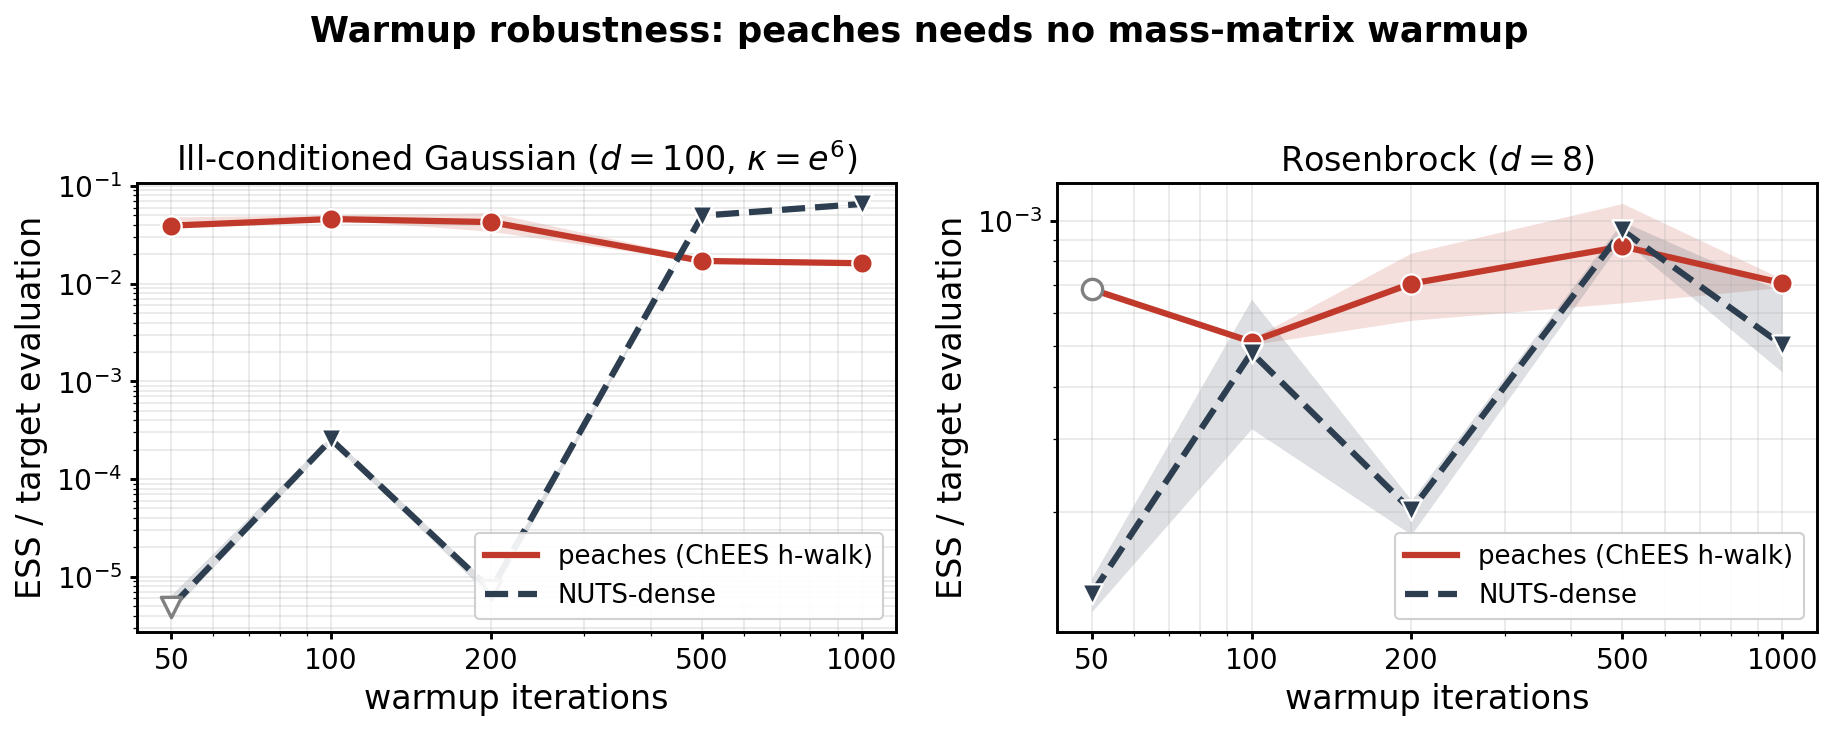
\includegraphics[width=\linewidth]{figs/pn_warmup.png}
\caption{ESS/eval vs.\ gradient-sampler warmup length, $8$ sampling seeds on a
fixed target. Line = median over the converged seeds; band = interquartile range
($25$--$75\%$) over those seeds (the IQR rather than min--max, because ChEES's
integration length is bimodal on the banana). Walkers: $128$ (Gaussian
$d{=}100$), $64$ (Rosenbrock $d{=}8$). \textsc{peaches} is
flat from warmup $50$ to $1000$; NUTS-dense
needs $\gtrsim\!500$ warmup steps to fit its mass matrix and is orders less
efficient below that (its $d{=}8$ Rosenbrock run at warmup $50$ barely converges,
shown hollow). Takeaway: because the metric is recomputed from the live ensemble
every step, \textsc{peaches} has no mass matrix to warm up --- the work NUTS
spends in a long target-dependent warmup, it gets for free.}
\label{fig:warmup}
\end{figure}

\paragraph{Setup.} Ill-conditioned Gaussian ($d{=}100$, $\kappa=e^6$, $128$
walkers, tag \texttt{warmf\_w$w$}) and Rosenbrock ($d{=}8$, $64$ walkers, tag
\texttt{warmfb\_w$w$}); warmup $\in\{50,100,200,500,1000\}$, production $5000$, $3$
seeds, ensemble ESS. NUTS uses a dense mass matrix (the standard choice on an
ill-conditioned target). \textsc{peaches} uses a $200$-step stretch pre-warmup
(\S\ref{sec:rec}) then its own warmup of the given length.

\paragraph{Result.} Because the preconditioner is recomputed from the live
ensemble every step, \textsc{peaches} needs no mass-matrix warmup: its ESS/eval
is flat at $\approx\!0.02$--$0.05$ (Gaussian) across all warmup lengths.
NUTS-dense must fit a $d(d{+}1)/2$-entry dense mass during warmup; at warmup $50$
its ESS/eval is $\approx\!5\times10^{-6}$ --- a factor $\sim\!10^4$ below
\textsc{peaches} --- and it becomes competitive only once warmup $\ge\!500$. The
same pattern holds on Rosenbrock. This is the practical face of ``the metric is
free'': the work NUTS spends in a long, target-dependent warmup, \textsc{peaches}
gets for nothing.

% =====================================================================
\section{Practical recommendation: a three-phase run}\label{sec:rec}

For \textsc{peaches} (and ensemble HMC generally) we recommend the following
workflow, which the benchmarks above all use:

\begin{enumerate}
\item[\textbf{1.}] \textbf{Stretch pre-warmup (gradient-free).} Run a short
\texttt{emcee}-style stretch move for $w_s$ iterations \emph{first}, from an
over-dispersed initialization. This is cheap (one log-density per walker, no
gradient) and affine-invariant, and it does two essential things: it moves the
ensemble \emph{mean} onto the typical set (a reasonable centre), and it shapes
the ensemble \emph{covariance} to the target's local geometry. This matters
because \textsc{peaches}'s preconditioner \emph{is} the empirical covariance: an
isotropic or collapsed initial cloud gives an ill-shaped metric, which in turn
collapses the dual-averaged step size and wastes the gradient warmup. A short
stretch phase suffices ($w_s\!\approx\!100$--$200$; benefit saturates quickly);
it uses no gradient and no knowledge of the target covariance.
\item[\textbf{2.}] \textbf{\textsc{peaches} warmup (gradient).} With the
ensemble now well-centred and well-shaped, run the \textsc{peaches} adapters:
\texttt{find\_init\_step\_size} for the initial $\epsilon$, dual averaging to the
target acceptance, and ChEES for the integration length. The
empirical-covariance metric is re-estimated each step, so no mass matrix is fit
here --- only the scalar $\epsilon$ and the length $L$.
\item[\textbf{3.}] \textbf{Production.} Freeze $(\epsilon,L)$ and the adapters
and collect samples. ESS/eval is measured here only.
\end{enumerate}

In the code this is exactly \texttt{(warm\_start $w_s$, warmup $w$,
num\_samples $N$)}. Phase 1 is the ensemble analogue of NUTS's mass-matrix
warmup, but gradient-free and target-agnostic; phase 2 is much shorter and more
robust than NUTS's because there is no mass matrix to converge
(\S\ref{sec:warmup}). Skipping phase 1 is the most common failure mode: without
it the worst-mixing direction is initialization-dependent and the step size can
collapse.

% =====================================================================
\section{Reproducibility}\label{sec:repro}

All runs go through \texttt{python -m benchmark.run} (one
\texttt{(target,dim,sampler,seed)} cell). Key flags:
\texttt{--target \{gaussian,rosenbrock\}}, \texttt{--dim}, \texttt{--sampler
\{peaches,stretch,nuts\}}, \texttt{--log-cond} ($\log\kappa$; $0$ + \texttt{--no-rotate}
for isotropic), \texttt{--n-chains}, \texttt{--warm-start} (stretch pre-warmup),
\texttt{--warmup}, \texttt{--num-samples}, \texttt{--target-accept},
\texttt{--max-L} (\textsc{peaches}), \texttt{--nuts-mass \{dense,diag,identity\}},
\texttt{--max-tree-depth}, \texttt{--seed}, \texttt{--tag}.

\begin{center}\small
\begin{tabular}{lllll}
\toprule
Experiment & target & sampler configs & walkers / warmup / prod. & tag \\
\midrule
Scaling (\S\ref{sec:scaling})
  & $N(0,I_d)$, $d{=}2$--$256$
  & \textsc{peaches} ($w_s{=}100$); \texttt{emcee}
  & $8d$ (floor $64$); $4$k/$5$k; emcee $3$k/$12$k & \texttt{scale3} \\
Scaling (\S\ref{sec:scaling})
  & Rosenbrock $d{=}2$--$32$
  & \textsc{peaches} $L_{\max}{=}512$; \texttt{emcee}
  & $8d$ (floor $64$); $8$k/$8$k & \texttt{rz8} \\
Bistability (\S\ref{sec:bistab})
  & Rosenbrock $d{=}2$ (\&\ $d{=}8$)
  & \textsc{peaches}, warmup/init sweeps
  & $64$/$256$; up to $32$k/$8$k & \texttt{b2\_*}, \texttt{rwarm\_w$w$} \\
Conditioning (\S\ref{sec:cond}a)
  & Gauss $d{=}50$, $\kappa{=}e^{2\text{-}8}$
  & \textsc{peaches}; \texttt{emcee}; NUTS \texttt{dense}/\texttt{identity}
  & $8d{=}400$; $1$k/$5$k & \texttt{condf\_lc$k$}, \texttt{condfid\_lc$k$} \\
Curvature (\S\ref{sec:cond}b)
  & Rosenbrock $d{\in}\{8,16,32\}$
  & \textsc{peaches} $L_{\max}{=}512$; \texttt{emcee}; NUTS \texttt{identity}
  & $8d$ (floor $64$); $8$k/$8$k & \texttt{rz8}, \texttt{rz8id} \\
Warmup (\S\ref{sec:warmup})
  & Gauss $d{=}100$ $\kappa{=}e^6$; Rosen $d{=}8$
  & \textsc{peaches} ($w_s{=}200$); NUTS \texttt{dense}
  & $400$/$64$; $\{50..1000\}$/$5$k & \texttt{warmf\_w$w$}, \texttt{warmfb\_w$w$} \\
\bottomrule
\end{tabular}
\end{center}
\noindent
The scaling sweep uses $5$ seeds ($3$ at $d{=}256$); the Rosenbrock scaling uses
$8$; the warmup experiment uses $6$; the rest use $3$. Per-dimension efficiency is
the median over the converged seeds ($\hat R\le1.03$); the warmup figure's band is
the interquartile range, all others are seed min--max. \textbf{All experiments are
scored with the ensemble-mean ESS} (\texttt{--fast-ess}), so the whole note uses a
single efficiency metric. Convergence ($\hat R$), bias, and std-error are stored
alongside ESS/eval in each
\texttt{metrics.json}. Figures are produced by
\texttt{benchmark/plot\_scaling2.py} (scaling) and
\texttt{benchmark/plot\_pn\_*.py} and \texttt{plot\_bistability.py} (the rest).

\paragraph{References.}
{\footnotesize
Beskos, Pillai, Roberts, Sanz-Serna, Stuart (2013), \emph{Optimal tuning of the
hybrid Monte Carlo algorithm}, Bernoulli 19(5A). \;
Goodman \& Weare (2010), \emph{Ensemble samplers with affine invariance}, Comm.\
App.\ Math.\ Comp.\ Sci.\ 5(1). \;
Foreman-Mackey, Hogg, Lang, Goodman (2013), \emph{emcee: the MCMC hammer}, PASP
125. \;
Hoffman \& Gelman (2014), \emph{The No-U-Turn Sampler}, JMLR 15. \;
Hoffman, Radul, Sountsov (2021), \emph{An adaptive-MCMC scheme for setting
trajectory lengths in Hamiltonian Monte Carlo}, AISTATS, PMLR 130.
}

\end{document}
